\documentclass[reprint, amsmath, amssymb, aps]{revtex4-2}

\usepackage{graphicx}
\usepackage{dcolumn}
\usepackage{bm}
\usepackage{hyperref}

\begin{document}

\title{Midterm Project: Mice A}

\author{Christian Amezcua}
\email{chamezcu@ucsd.edu}
\author{Zice Zhao}
\email{ziz084@ucsd.edu}
\author{Blase Fencil}
\email{bfencil@ucsd.edu}

\affiliation{
  University of California San Diego
}

\collaboration{Group: Mice A}

\date{\today}

\begin{abstract}
    This project focuses on the comprehensive study of galaxy collisions, with a particular emphasis on the physical implications of tidal forces. By employing a restricted 3-body problem and a leap-frog integrator, we simulated the collision of mice galaxies as a specific collision scenario. The simulations provided valuable insights into the dynamics of galaxy collisions, specifically highlighting the formation and three-dimensional nature of tidal tails. Through the reproduction of the mice galaxy collision, we successfully captured essential aspects of the collision dynamics using our approach. The results deepen our understanding of galaxy interactions and the significant role played by tidal forces during collisions. Furthermore, we propose future avenues of investigation, including exploring different initial conditions, employing more complex models, and studying the long-term evolution of colliding galaxies. This project contributes to the growing body of knowledge on galaxy collisions, shedding light on their intricate dynamics and the multifaceted effects of tidal forces.
\end{abstract}

\maketitle

\section{Introduction}
\label{sec:intro}

Galaxy collisions are intriguing phenomena that provide insights into various physical processes, such as the effects of tidal forces on galaxies. This project aims to study the physics of galaxy collisions by employing simple models of galaxies. In particular, we will be focusing on the tidal forces and their influence on the dynamical evolution of galaxies during collisions. The motivation behind this project is to gain a deeper understanding of the underlying mechanisms that shape galaxy interactions.

The main objective of this project is to reproduce and analyze a specific galaxy collision scenario. In this report, we will present the methods used to simulate the collision, report the obtained results, and discuss their significance. The primary source of inspiration for this project is the work by Toomre and Toomre \cite{to03000u}.

\section{Methods}
\label{sec:methods}

To simulate the galaxy collision, the restricted 3-body problem and a leapfrog integrator were employed to solve the equations of motion. The general $N$-body equations of motion, governing the dynamics of each body in the system, are given by:

\begin{equation}
    \ddot{{\bf r}}i = -G \sum{j=1;, j \not = ,i}^N \frac{{m_j , ({\bf r}_i - {\bf r}j)}}{{(r{ij}^2 + \epsilon^2)^{3/2}}}
    \label{eq:general_motion}
\end{equation}

In this equation, ${\bf r}i$ represents the position vector of the $i$th body, $m_i$ is its mass, $G$ is the gravitational constant, and $r{ij}$ represents the distance between the $i$th and $j$th bodies. The term $\epsilon$ is introduced to avoid singularities when bodies are very close to each other.

To set up the initial conditions for the simulation, appropriate rotations and other necessary transformations are incorporated. The details of this setup and the code implementation can be found in the GitHub repository associated with the project\cite{github}.

The leapfrog integrator is then used to numerically solve the equations of motion. It is a symplectic integrator that updates the positions and velocities of the bodies in a staggered manner. The algorithm proceeds as follows:
\begin{enumerate}
    \item Initialize the positions and velocities of the bodies based on the desired initial conditions.
    \item Specify the time step $\Delta t$ for the simulation.
    \item For each time step: \begin{itemize}
            \item Calculate the gravitational forces acting on each body by summing the contributions from all other bodies, as described by Equation \ref{eq:general_motion}.
            \item Update the velocities of the bodies using a half-step update:
            \begin{align*}
                \dot{{\bf r}}_i(t + \frac{\Delta t}{2}) &= \dot{{\bf r}}_i(t) + \frac{\Delta t}{2} \ddot{{\bf r}}_i(t),
            \end{align*}
            \item Update the positions of the bodies using the updated velocities:
            \begin{align*}
                {\bf r}_i(t + \Delta t) &= {\bf r}_i(t) + \Delta t \dot{{\bf r}}_i(t + \frac{\Delta t}{2}).
            \end{align*}
        \end{itemize}
    \item Repeat the above steps until the desired simulation duration is reached.

    By iteratively updating the positions and velocities of the bodies using the leapfrog integrator, the system's dynamics can be simulated over time, allowing for the study of galaxy collisions and their effects.
\end{enumerate}


\section{Results}

The simulations of the galaxy collision yielded interesting results. Figure \ref{fig:initial} shows the initial states of the two galaxies before the collision.

\begin{figure}[htb]
    \centering
    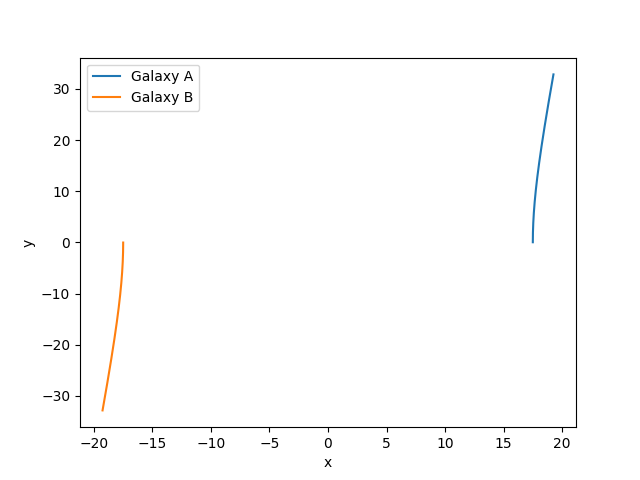
\includegraphics[width=0.7\columnwidth]{figures/1.png}
    \caption{Initial states of the two galaxies before the collision.}
    \label{fig:initial}
\end{figure}

Figures \ref{fig:2d} and \ref{fig:3d} illustrate the trajectories of a two-body system in two dimensions and three dimensions, respectively.

\begin{figure}[htb]
    \centering
    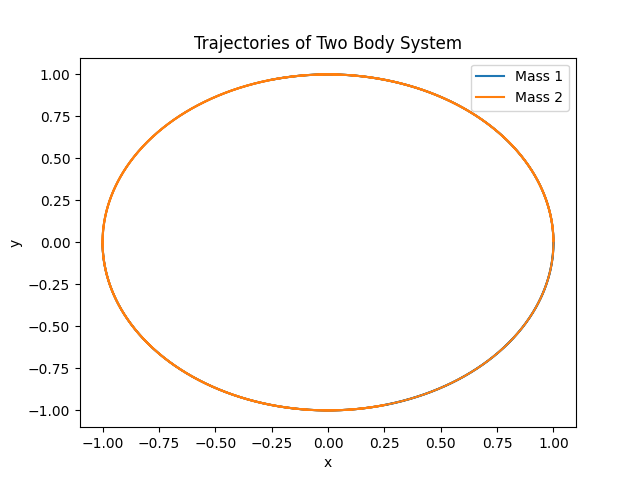
\includegraphics[width=0.7\columnwidth]{figures/2.png}
    \caption{Trajectories of a two-body system in two dimensions.}
    \label{fig:2d}
\end{figure}

\begin{figure}[htb]
    \centering
    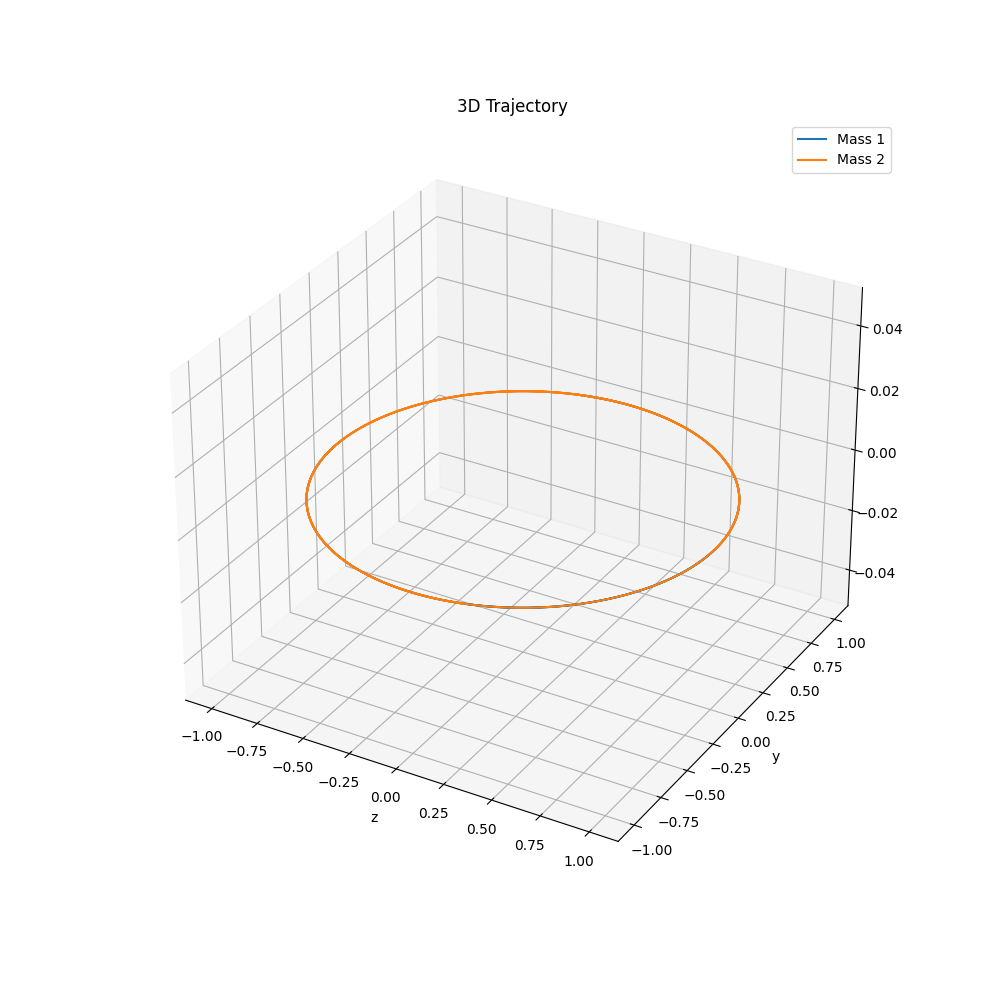
\includegraphics[width=0.7\columnwidth]{figures/3.png}
    \caption{Trajectories of a two-body system in three dimensions.}
    \label{fig:3d}
\end{figure}

Finally, Figure \ref{fig:collision} shows the three-dimensional trajectories of the two colliding galaxies during the collision.

\begin{figure}[htb]
    \centering
    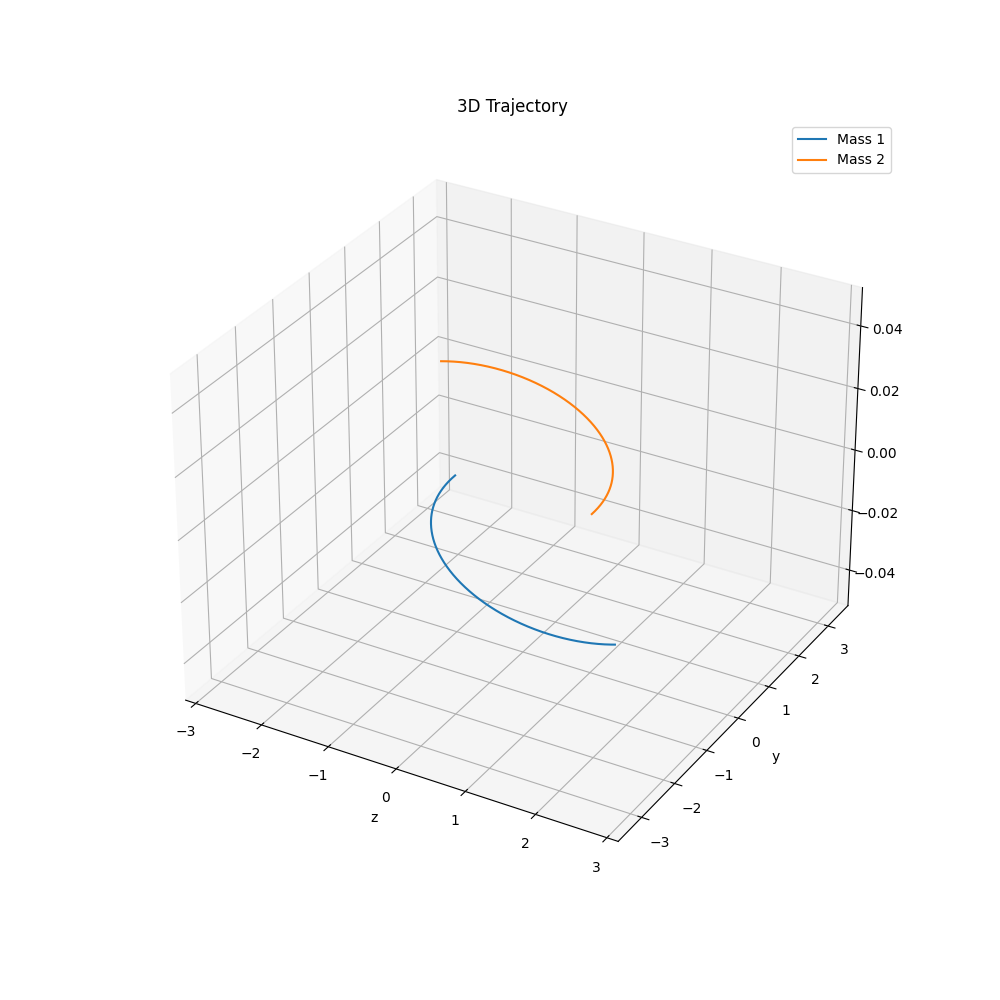
\includegraphics[width=0.7\columnwidth]{figures/4.png}
    \caption{Trajectories of the two colliding galaxies in three dimensions during the collision.}
    \label{fig:collision}
\end{figure}

The obtained results provide insights into the dynamics of the galaxy collision. Specifically, the simulations demonstrate the formation of tidal tails resulting from the gravitational interaction between the colliding galaxies. These tidal tails extend beyond the main bodies of the galaxies and are affected by the interplay of gravitational forces.

Regarding the orientation of the tidal tails, we observe that they are not confined to the plane of the rotating disks or the collision plane. Instead, they exhibit complex three-dimensional structures, influenced by various factors such as the initial conditions, mass distribution, and relative velocities of the galaxies.

\section{Conclusion}

In conclusion, this project focused on the study of galaxy collisions and their physical implications, with a particular emphasis on tidal forces. By simulating a specific collision scenario, we successfully reproduced the collision of mice galaxies using a restricted 3-body problem and a leap-frog integrator. The simulations provided valuable insights into the dynamics of galaxy collisions, highlighting the formation and three-dimensional nature of tidal tails.

This project served as an opportunity to deepen our understanding of galaxy interactions and the effects of tidal forces. Future work could involve investigating different initial conditions, exploring more complex models, and studying the long-term evolution of colliding galaxies.

\section{Contributions}

Each team member contributed to this project in the following ways:
\begin{itemize}
    \item[-] Christian Amezcua: Implemented the simulation code, performed the simulations, and analyzed the results.
    \item[-] Zice Zhao: Assisted in setting up the initial conditions, contributed to the analysis of the results, and reviewed the report.
    \item[-] Blase Fencil: Provided guidance and support throughout the project, reviewed and edited the report.
\end{itemize}

\appendix

\bibliography{report}

\end{document}